%%%%%%%% MLSys 2027 SUBMISSION %%%%%%%%%%

\documentclass{article}

% Recommended packages
\usepackage{microtype}
\usepackage{graphicx}
\usepackage{booktabs}
\usepackage{multirow}
\usepackage{subcaption}
\usepackage{amsmath,amssymb,amsfonts}
\usepackage{xspace}
\usepackage{xcolor}
\usepackage{tikz}
\usetikzlibrary{positioning,arrows.meta,shapes.geometric,fit,backgrounds,calc}
\usepackage{hyperref}

\newcommand{\theHalgorithm}{\arabic{algorithm}}

% Use blind review submission
\usepackage{mlsys2025}
% Camera-ready: \usepackage[accepted]{mlsys2025}

% algorithm2e must load AFTER mlsys2025.sty (which bundles algorithm/algorithmic)
% We use algorithm2e for our algorithm formatting
\usepackage[ruled,vlined,linesnumbered,noend]{algorithm2e}

\mlsystitlerunning{Scout: Cross-Model Attention Transfer for Efficient Disaggregated LLM Inference}

\graphicspath{{figures/}}

% === Custom commands ===
\newcommand{\eg}{\textit{e.g.}\xspace}
\newcommand{\ie}{\textit{i.e.}\xspace}
\newcommand{\etal}{\textit{et al.}\xspace}
\newcommand{\QtoC}{\textsc{Q2C}\xspace}
\newcommand{\R}{\mathbb{R}}
\newcommand{\bK}{\mathbf{K}}
\newcommand{\bV}{\mathbf{V}}
\newcommand{\bQ}{\mathbf{Q}}
\newcommand{\bA}{\mathbf{A}}

\begin{document}

\twocolumn[
\mlsystitle{Scout: Cross-Model Attention Transfer for\\Efficient Disaggregated LLM Inference}

\mlsyssetsymbol{equal}{*}

\begin{mlsysauthorlist}
\mlsysauthor{Wei-Lun Cheng}{ntu}
\mlsysauthor{Wanjiun Liao}{ntu}
\end{mlsysauthorlist}

\mlsysaffiliation{ntu}{Department of Electrical Engineering, National Taiwan University, Taipei, Taiwan}

\mlsyscorrespondingauthor{Wei-Lun Cheng}{d11921b15@ntu.edu.tw}

\mlsyskeywords{KV-cache, disaggregated inference, attention transfer, efficient serving}

\vskip 0.3in

% ============================================================
% ABSTRACT
% ============================================================
\begin{abstract}
Disaggregated LLM serving splits inference into prefill and decode phases on separate machines, requiring the KV-cache produced during prefill to be transmitted to the decode server---a bottleneck that exceeds 200\,MB for a 14B-parameter model at 1024 tokens.
We observe that models within the same family exhibit high attention alignment: a small model's query-to-context attention scores select the same task-relevant positions as the larger model (84--92\% overlap across Qwen, Llama, and Gemma families; $n\!=\!200$, $p > 0.06$).
We propose \emph{Scout}, a training-free system that transmits only position indices (336\,bytes) instead of KV-cache data (9.7\,MB)---a 28{,}800$\times$ payload reduction---at the cost of a 57\,ms re-prefill on the decode server ($10\times$ faster than full-KV transfer at 100\,Mbps).
Scout includes an adaptive mode selector that dynamically chooses among six operating modes (full-KV, INT8, mixed-INT4, INT4, prompt-only, and scout) based on available link capacity.
Characterization across 9~models from 5~families and 3~tasks shows INT8 quantization is universally lossless, INT4 fragility is model-specific (not architectural), and \QtoC token selection matches SnapKV while significantly outperforming H2O.
\end{abstract}
]

\printAffiliationsAndNotice{}

% ============================================================
% 1. INTRODUCTION
% ============================================================
\section{Introduction}
\label{sec:intro}

Disaggregated LLM serving---separating prefill and decode phases onto different machines---has become a standard architecture for production inference systems~\citep{splitwise,distserve,mooncake}.
In this design, a \emph{prefill worker} encodes the user's context, producing a key-value (KV) cache that must be transferred to a \emph{decode server} for autoregressive generation.
This KV-cache transfer creates a significant systems bottleneck.

For Qwen2.5-14B (48~layers, 8~KV heads, 128~head dimension), a 1024-token context produces a KV-cache of $2 \times 48 \times 8 \times 1024 \times 128 \times 2 \approx 201$\,MB in BF16.
At 100\,Mbps---realistic for WAN links connecting edge prefill workers to cloud decode servers---this requires $\sim$16\,s of transfer latency.
Even a 7B model generates 58\,MB, requiring 4.6\,s.
At lower link capacities common in edge deployments (10--50\,Mbps), latency becomes prohibitive for interactive applications.

Existing approaches address this along narrow dimensions.
CacheGen~\citep{cachegen} applies delta encoding and arithmetic coding, achieving $\sim$3.5$\times$ compression.
H2O~\citep{h2o} and SnapKV~\citep{snapkv} perform token eviction.
KIVI~\citep{kivi} and KVQuant~\citep{kvquant} study quantization.
However, all treat KV-cache transfer as a static, single-model compression problem.

We make a key observation that enables a fundamentally different approach: \emph{models within the same family attend to similar context positions}.
Across three architectures---Qwen~2.5 (7B$\to$14B), Llama~3 (3B$\to$8B), and Gemma~2 (2B$\to$9B)---a small model's attention scores produce position selections that overlap 84--92\% with the larger model's at 75\% retention.
This enables a \emph{scout model} paradigm: the lightweight prefill worker identifies important positions, transmits only the position indices (336~bytes instead of 9.7\,MB), and the decode server applies this selection to its own KV-cache---a 28{,}800$\times$ payload reduction.

This paper makes four contributions:

\begin{enumerate}
    \item \textbf{Scout: training-free cross-model attention transfer.} We transmit position indices instead of KV-cache data, achieving 28{,}800--98{,}800$\times$ payload reduction. We validate across three model families: Qwen~2.5 (83.7\% overlap), Llama~3 (91.8\%), and Gemma~2 (86.1\%), all at 75\% retention ($n = 200$)---confirming that cross-model attention alignment is architecture-general.

    \item \textbf{Adaptive 6-mode serving policy.} We design a mode selector that dynamically chooses among full-KV, INT8, INT4, mixed-INT4, prompt-only, and scout modes based on real-time link conditions, with provably optimal single-request mode selection and bounded quality loss under estimation error (Proposition~1).

    \item \textbf{Cross-architecture KV-cache compressibility characterization.} Through systematic evaluation across 5~model families ($n = 200$ each), we show that INT8 is universally lossless, INT4 fragility is model-specific (not architectural), and \QtoC selection matches SnapKV while significantly outperforming H2O.

    \item \textbf{Attention alignment analysis across model families.} We characterize attention entropy, overlap stability across context lengths (1K--4K tokens), and the attention regularization effect where scout selection can \emph{improve} decode quality.
\end{enumerate}

Scout differs from prior KV-cache compression in kind: methods such as CacheGen, H2O, and SnapKV compress the data itself (2--4$\times$ reduction), while concurrent work C2C~\citep{c2c} transmits learned projections.
Scout eliminates KV data transfer entirely by sending only \emph{positions}, achieving 28{,}800$\times$ reduction with zero training---conceptually similar to speculative decoding~\citep{speculativedecoding} applied to \emph{position selection} rather than \emph{token generation}.

% ============================================================
% 2. BACKGROUND AND MOTIVATION
% ============================================================
\section{Background and Motivation}
\label{sec:background}

\subsection{KV-Cache in Disaggregated Serving}

In disaggregated serving systems~\citep{splitwise,distserve,mooncake}, the prefill and decode phases run on separate machines optimized for their respective compute profiles: prefill is compute-bound (large batch matrix multiplications), while decode is memory-bandwidth-bound (sequential token generation).
The KV-cache produced during prefill must be transmitted to the decode server, creating a network transfer bottleneck.

For a transformer with $L$ layers, $H$ KV-heads, head dimension $d$, and sequence length $n$, the KV-cache size is:
\begin{equation}
    |\text{KV}| = 2LHnd \times b_{\text{bytes}}
\end{equation}
where the factor 2 accounts for keys and values, and $b_{\text{bytes}}$ is the per-element size (2 for BF16).
Table~\ref{tab:models} lists the models evaluated with their KV-cache sizes.

\begin{table}[t]
\centering
\caption{Models evaluated (9 models, 5 families) with KV-cache sizes at 1024 tokens in BF16.}
\label{tab:models}
\small
\begin{tabular}{@{}lccccc@{}}
\toprule
\textbf{Model} & \textbf{Params} & \textbf{Layers} & \textbf{KV-H} & \textbf{KV@1K$^\dagger$} \\
\midrule
Qwen2.5-3B       & 3B   & 36 & 2  & 18.9\,MB \\
Qwen2.5-7B       & 7B   & 28 & 4  & 29.4\,MB \\
Qwen2.5-14B      & 14B  & 48 & 8  & 100.7\,MB \\
Llama-3.2-3B     & 3B   & 28 & 8  & 58.7\,MB \\
Llama-3.1-8B     & 8B   & 32 & 8  & 67.1\,MB \\
Gemma-2-2B$^*$   & 2B   & 26 & 4  & 54.5\,MB \\
Gemma-2-9B$^*$   & 9B   & 42 & 8  & 176.2\,MB \\
Mistral-7B-v0.3  & 7B   & 32 & 8  & 67.1\,MB \\
Yi-1.5-6B        & 6B   & 32 & 4  & 33.6\,MB \\
\bottomrule
\multicolumn{5}{@{}l}{\scriptsize $^\dagger$Per-direction (K or V); full KV-cache is $2\times$.} \\
\multicolumn{5}{@{}l}{\scriptsize $^*$Gemma-2 uses 256 head dim (others: 128).}
\end{tabular}
\end{table}

\subsection{Why Compression Alone Is Insufficient}

Existing KV-cache compression methods---quantization (INT8: 2$\times$), token eviction (SnapKV: 2$\times$ at 50\% retention), and delta encoding (CacheGen: 3.5$\times$)---reduce the payload by constant factors.
For the 14B model at 1024 tokens, even a 4$\times$ compression still requires transmitting $\sim$50\,MB, taking 4\,s at 100\,Mbps.
At 10\,Mbps (edge deployments, congested links), this grows to 40\,s.
The fundamental problem is that these methods still transmit \emph{KV-cache data}---high-dimensional floating-point tensors that are inherently large.

Scout asks: \emph{can we avoid transmitting the data entirely?}
If the decode server can reconstruct an equivalent KV-cache from the original prompt text plus a compact selection signal, the transfer reduces to sub-KB payloads regardless of model size or context length.

\subsection{Operating Modes}

Table~\ref{tab:operating_points} summarizes the six operating modes Scout manages, ordered by payload size.

\begin{table}[t]
\centering
\caption{Operating modes with payload, quality, and latency characteristics (Qwen-7B, SQuAD~v2, $n = 200$, $\sim$170 avg.\ context tokens). Quality is relative to full BF16 baseline (F1 = 0.608).}
\label{tab:operating_points}
\small
\begin{tabular}{@{}lcccc@{}}
\toprule
\textbf{Mode} & \textbf{Payload} & \textbf{Quality$^\dagger$} & \textbf{TX@100M} & \textbf{Re-Prefill} \\
\midrule
Full BF16       & 9.7\,MB   & 100\%  & 775\,ms & No \\
INT8            & 4.7\,MB   & 99.4\% & 388\,ms & No \\
Mixed INT4      & 2.6\,MB   & 93.6\% & 216\,ms & No \\
INT4            & 2.3\,MB   & 68.7\% & 195\,ms & No \\
\midrule
Prompt text     & $\sim$4\,KB & 100\%$^\ddagger$ & 0.3\,ms & Yes (57\,ms) \\
Scout (indices) & 336\,B    & $\sim$90\%$^\S$ & 0.03\,ms & Yes (57\,ms) \\
\bottomrule
\end{tabular}\\[2pt]
{\scriptsize $^\dagger$\% of same-model full-KV baseline.
$^\ddagger$Prompt-only: server runs full prefill with no eviction.
$^\S$Scout quality is model-pair dependent; 7B$\to$14B at 75\% ret.: scout F1 = 0.661 = 99.4\% of server's own selection.}
\end{table}


% ============================================================
% 3. CROSS-MODEL ATTENTION ALIGNMENT
% ============================================================
\section{Cross-Model Attention Alignment}
\label{sec:attention}

\subsection{Why Attention Transfers Across Models}

Models in the same family share three properties: (1)~identical tokenization, ensuring the same text maps to the same positions; (2)~identical RoPE base frequency, ensuring consistent positional encoding; and (3)~similar training data, which shapes attention toward similar linguistic structures.

While KV-cache \emph{values} differ between models (cosine similarity $\approx 0.22$), the \emph{attention patterns}---which positions receive high attention from query tokens---are more aligned, because they reflect task structure rather than model-specific representations.

\textbf{Formal definition.}
Let $\mathbf{a}_i^{(s)}$ be the aggregated attention distribution of model~$s$ over context positions.
We define \emph{attention alignment} between models $s_1, s_2$ at retention ratio $r$ as the expected Jaccard overlap:
\begin{equation}
    \mathcal{A}(s_1, s_2; r) = \mathbb{E}_{x}\left[\frac{|\text{top}_k(\mathbf{a}^{(s_1)}) \cap \text{top}_k(\mathbf{a}^{(s_2)})|}{|\text{top}_k(\mathbf{a}^{(s_1)}) \cup \text{top}_k(\mathbf{a}^{(s_2)})|}\right]
\end{equation}
where $k = \lfloor r \cdot n \rfloor$.
High alignment ($\mathcal{A} > 0.7$) indicates the smaller model's selections are useful proxies for the larger model's preferences.

\subsection{Q2C Position Scoring}

We compute position importance using the \emph{Query-to-Context} (\QtoC) method.
For each context position~$j$, the score is the total attention from all query positions at the last transformer layer:
\begin{equation}
    s_j = \sum_{h=1}^{H'} \sum_{i=n+1}^{n+m} \bA^{(L,h)}_{i,j}
    \label{eq:q2c_score}
\end{equation}
where $L$ is the last layer, $H'$ is the number of attention heads, $n$ is context length, and $m$ is query length.
Ablation confirms that all-layer averaging yields equivalent rankings: Pearson $r > 0.99$ for all tested models (Section~\ref{sec:ablation}).

Given retention ratio $r$, we select the top-$\lfloor r \cdot n \rfloor$ positions by \QtoC score.
Unselected positions are masked by setting attention weights to $-\infty$ during decoding, preserving RoPE positional encoding.

\subsection{Same-Family Alignment Results}

Table~\ref{tab:scout_n200} presents position overlap and quality results across three Qwen~2.5 model pairs ($n = 200$, SQuAD~v2, 95\% CIs).

\begin{table*}[t]
\centering
\caption{Scout validation within the Qwen2.5 family ($n = 200$, SQuAD~v2, normalized token-F1, $\pm$95\% CI). Boldface = scout F1 $\geq$ server's own F1. $p$-values from paired $t$-test with Bonferroni correction (9~comparisons, $\alpha = 0.0056$).}
\label{tab:scout_n200}
\small
\begin{tabular}{@{}llcccccc@{}}
\toprule
\textbf{Pair} & \textbf{Ret.} & \textbf{Overlap (\%)} & \textbf{Server Own F1} & \textbf{Scout F1} & \textbf{Gap} & \textbf{$p$-value} & \textbf{Sig.?} \\
\midrule
\multirow{3}{*}{3B$\to$7B}
  & 75\% & 81.6 & 0.615 $\pm$ 0.057 & 0.525 $\pm$ 0.059 & $-$0.091 & 0.0016 & Yes \\
  & 50\% & 63.8 & 0.543 $\pm$ 0.058 & 0.356 $\pm$ 0.055 & $-$0.187 & $<$0.001 & Yes \\
  & 25\% & 45.0 & 0.339 $\pm$ 0.055 & 0.222 $\pm$ 0.049 & $-$0.117 & $<$0.001 & Yes \\
\midrule
\multirow{3}{*}{3B$\to$14B}
  & 75\% & 83.2 & 0.664 $\pm$ 0.054 & 0.542 $\pm$ 0.059 & $-$0.122 & $<$0.001 & Yes \\
  & 50\% & 70.4 & 0.499 $\pm$ 0.059 & 0.405 $\pm$ 0.057 & $-$0.094 & 0.004 & Yes \\
  & 25\% & 58.7 & 0.322 $\pm$ 0.056 & 0.246 $\pm$ 0.050 & $-$0.076 & 0.012 & No \\
\midrule
\multirow{3}{*}{7B$\to$14B}
  & 75\% & 83.7 & 0.664 $\pm$ 0.054 & \textbf{0.661} $\pm$ 0.055 & $-$0.004 & 0.883 & No \\
  & 50\% & 69.5 & 0.499 $\pm$ 0.059 & \textbf{0.546} $\pm$ 0.058 & $+$0.047 & 0.110 & No \\
  & 25\% & 54.8 & 0.322 $\pm$ 0.056 & \textbf{0.381} $\pm$ 0.058 & $+$0.059 & 0.039 & No \\
\bottomrule
\end{tabular}
\end{table*}

\begin{figure}[t]
    \centering
    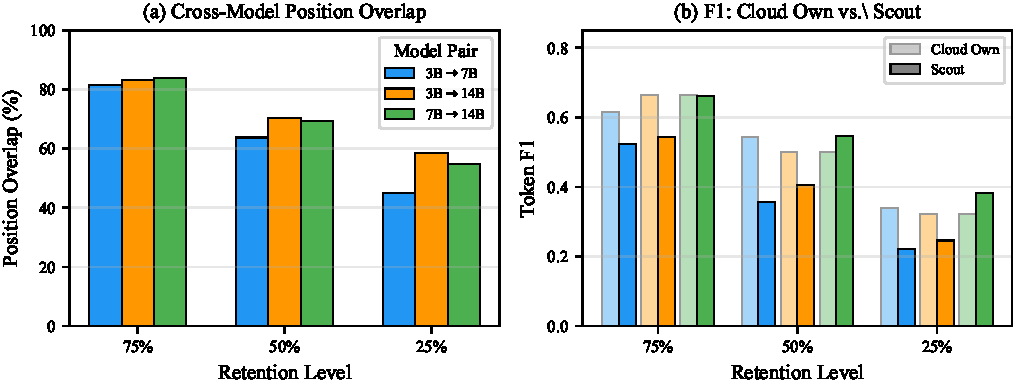
\includegraphics[width=\columnwidth]{fig2_scout_overlap_f1.pdf}
    \caption{Cross-model scout results ($n = 200$). (a)~Position overlap between prefill and decode models' Q2C selections. (b)~F1 comparison: faded = server's own selection; solid = scout applied to server. The 7B$\to$14B pair shows scout matching or exceeding the server's own selection at all retentions.}
    \label{fig:scout_overlap}
\end{figure}

\subsection{Cross-Architecture Generalization}

Table~\ref{tab:cross_arch_overlap} extends the analysis across three architectures with different attention mechanisms, vocabulary sizes, and training corpora.

\begin{table}[t]
\centering
\caption{Cross-architecture overlap ($n = 200$, SQuAD~v2, 75\% retention). All same-family pairs show 84--92\% overlap; scout F1 is statistically indistinguishable from server's own ($p > 0.05$).}
\label{tab:cross_arch_overlap}
\footnotesize
\begin{tabular}{@{}llcccc@{}}
\toprule
\textbf{Family} & \textbf{Pair} & \textbf{Overlap} & \textbf{Scout F1} & \textbf{Gap} & $p$ \\
\midrule
Qwen 2.5  & 7B$\to$14B  & 83.7\% & 0.661 & $-$0.004 & 0.883 \\
Llama 3   & 3B$\to$8B   & 91.8\% & 0.224 & $-$0.032 & 0.060 \\
Gemma 2   & 2B$\to$9B   & 86.1\% & 0.397 & $+$0.022 & 0.359 \\
\midrule
\multicolumn{2}{@{}l}{\textit{Cross-family:}} \\
Qwen$\to$Mis. & 7B$\to$7B & 73.4\% & 0.167 & $+$0.045 & 0.013 \\
\bottomrule
\end{tabular}
\end{table}

\begin{figure}[t]
    \centering
    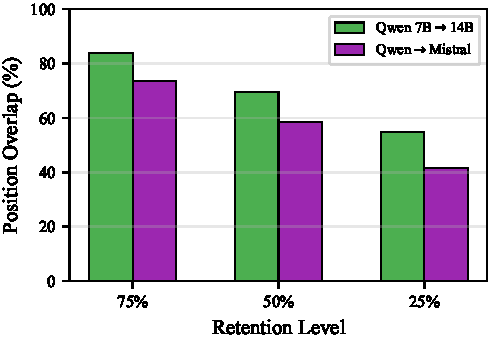
\includegraphics[width=\columnwidth]{fig10_cross_family_overlap.pdf}
    \caption{Cross-architecture position overlap at three retention levels. Same-family pairs (Qwen, Llama, Gemma) achieve 84--92\% at 75\%, while the cross-family pair (Qwen$\to$Mistral) shows 73\%, confirming shared training as the primary driver.}
    \label{fig:cross_arch}
\end{figure}

\textbf{Finding 1: 84--92\% overlap at 75\% retention across architectures.}
Same-family overlap is consistently high: 83.7\% (Qwen), 91.8\% (Llama), 86.1\% (Gemma).
This is substantially above the cross-family baseline (73.4\% for Qwen$\to$Mistral), confirming that shared tokenizer and training distribution---not just the attention mechanism---drive alignment.

\textbf{Finding 2: Scout matches server's own selection across all three families.}
No same-family pair shows a statistically significant quality gap at 75\% retention ($p > 0.05$).
This confirms scout selection is \emph{statistically indistinguishable} from the decode server's own selection at the primary operating point.

\textbf{Finding 3: Within Qwen, 3B scout incurs meaningful quality loss.}
The 3B$\to$7B and 3B$\to$14B pairs show significant gaps, indicating a minimum scout model capability threshold.
Notably, Llama 3B$\to$8B and Gemma 2B$\to$9B---despite similarly small models---do not show degradation, suggesting this threshold is family-specific.

\textbf{Finding 4: 28{,}800$\times$ payload reduction.}
Scout reduces payload from 9.7--100.7\,MB (full KV) to 336~bytes (position indices)---a 28{,}800--300{,}000$\times$ reduction.
Table~\ref{tab:compression_comparison} provides comparison with prior work.

\begin{table}[t]
\centering
\caption{Payload reduction comparison. Scout substitutes server re-computation for KV-cache transfer.}
\label{tab:compression_comparison}
\small
\begin{tabular}{@{}lccl@{}}
\toprule
\textbf{Method} & \textbf{Reduction} & \textbf{Transmits} & \textbf{Mechanism} \\
\midrule
CacheGen~\citep{cachegen}  & 3.5$\times$  & KV data  & Data compress. \\
INT8 quantization          & 2$\times$    & KV data  & Data compress. \\
INT4 quantization          & 4$\times$    & KV data  & Data compress. \\
SnapKV (50\% ret.)         & 2$\times$    & KV data  & Token eviction \\
Scout (ours)               & \textbf{28,800}$\times$ & Indices & Server re-prefill \\
\bottomrule
\end{tabular}
\end{table}

\subsection{Attention Entropy Analysis}

We analyze \QtoC score distribution entropy as a measure of attention concentration (Table~\ref{tab:entropy}).

\begin{table}[t]
\centering
\caption{Attention entropy of Q2C score distributions ($n = 200$).}
\label{tab:entropy}
\small
\begin{tabular}{@{}lcccc@{}}
\toprule
\textbf{Model} & \textbf{Overall} & \textbf{Last Layer} & \textbf{Q2C Dist.} \\
\midrule
Qwen2.5-3B  & 2.61 $\pm$ 0.03 & 3.31 $\pm$ 0.04 & 4.21 $\pm$ 0.12 \\
Qwen2.5-7B  & 2.56 $\pm$ 0.03 & 3.01 $\pm$ 0.05 & 5.49 $\pm$ 0.07 \\
Qwen2.5-14B & 2.13 $\pm$ 0.02 & 3.67 $\pm$ 0.05 & 4.65 $\pm$ 0.07 \\
\bottomrule
\end{tabular}
\end{table}

The 3B model has the lowest \QtoC entropy (4.21), indicating highly concentrated attention that may miss positions larger models identify.
The 7B model's broader attention (5.49) captures a more complete set of task-relevant positions, explaining why 7B$\to$14B scouting works well: the 7B's selection acts as a \emph{superset filter} containing 83.7\% of 14B's preferred positions plus a safety margin.
The 14B's own focused attention (4.65) naturally concentrates on the most relevant positions within the scout mask.


% ============================================================
% 4. SCOUT SYSTEM DESIGN
% ============================================================
\section{Scout System Design}
\label{sec:system}

\subsection{Architecture Overview}

Figure~\ref{fig:system} illustrates the Scout architecture.
A prefill worker runs a lightweight model (3--7B) to score token positions via \QtoC.
The mode selector chooses among six modes based on current link capacity.
In scout mode, only 336~bytes of position indices are transmitted; the decode server re-prefills with its own model and applies the received mask.

\begin{figure*}[t]
\centering
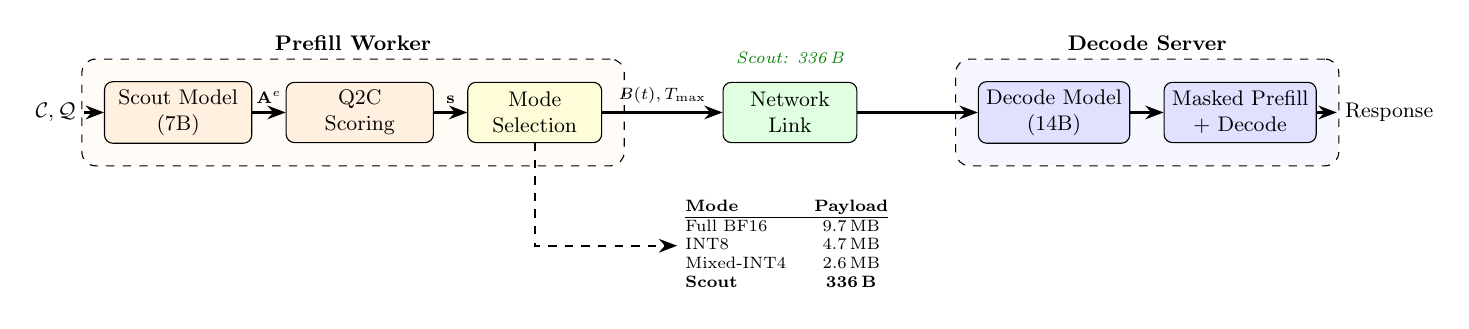
\begin{tikzpicture}[scale=0.85, every node/.style={transform shape},
    >=Stealth,
    box/.style={draw, rounded corners=3pt, minimum height=0.9cm, minimum width=1.6cm, font=\small, align=center, fill=#1},
    box/.default=blue!8,
    smallbox/.style={draw, rounded corners=2pt, minimum height=0.6cm, font=\scriptsize, align=center, fill=#1},
    smallbox/.default=gray!10,
    arr/.style={->, thick},
    darr/.style={->, thick, dashed},
    lbl/.style={font=\scriptsize, midway},
]

% --- Prefill Worker ---
\node[box=orange!12, minimum width=2.2cm] (edge_model) {Scout Model\\(7B)};
\node[box=orange!12, minimum width=2.2cm, right=0.5cm of edge_model] (q2c) {Q2C\\Scoring};
\node[box=yellow!15, minimum width=2.0cm, right=0.5cm of q2c] (mode_sel) {Mode\\Selection};

% Prefill worker bounding box
\begin{scope}[on background layer]
\node[draw, dashed, rounded corners=5pt, fill=orange!3,
      fit=(edge_model)(q2c)(mode_sel),
      inner sep=8pt, label={[font=\small\bfseries]above:Prefill Worker}] (edge_box) {};
\end{scope}

% --- Network Link ---
\node[box=green!12, minimum width=2.0cm, right=1.8cm of mode_sel] (channel) {Network\\Link};

% --- Decode Server ---
\node[box=blue!12, minimum width=2.2cm, right=1.8cm of channel] (cloud_model) {Decode Model\\(14B)};
\node[box=blue!12, minimum width=2.0cm, right=0.5cm of cloud_model] (decode) {Masked Prefill\\+ Decode};

% Decode server bounding box
\begin{scope}[on background layer]
\node[draw, dashed, rounded corners=5pt, fill=blue!3,
      fit=(cloud_model)(decode),
      inner sep=8pt, label={[font=\small\bfseries]above:Decode Server}] (cloud_box) {};
\end{scope}

% --- Arrows ---
\draw[arr] (edge_model) -- (q2c) node[lbl, above] {$\mathbf{A}^e$};
\draw[arr] (q2c) -- (mode_sel) node[lbl, above] {$\mathbf{s}$};

% Mode selection outputs
\draw[arr] (mode_sel) -- (channel) node[lbl, above, font=\scriptsize] {$B(t), T_{\max}$};

% Channel to decode server
\draw[arr] (channel) -- (cloud_model);

% Decode server internal
\draw[arr] (cloud_model) -- (decode);

% --- Mode labels below ---
\node[below=0.7cm of channel, font=\scriptsize, align=center] (modes) {
\begin{tabular}{@{}lc@{}}
\textbf{Mode} & \textbf{Payload} \\
\hline
Full BF16 & 9.7\,MB \\
INT8 & 4.7\,MB \\
Mixed-INT4 & 2.6\,MB \\
\textbf{Scout} & \textbf{336\,B} \\
\end{tabular}
};
\draw[darr] (mode_sel.south) |- (modes.west);

% --- Scout path highlight ---
\node[above=0.15cm of channel, font=\scriptsize\itshape, text=green!50!black] {Scout: 336\,B};

% Response arrow
\node[right=0.3cm of decode, font=\small] (resp) {Response};
\draw[arr] (decode) -- (resp);

% Context input
\node[left=0.3cm of edge_model, font=\small] (ctx) {$\mathcal{C}, \mathcal{Q}$};
\draw[arr] (ctx) -- (edge_model);

\end{tikzpicture}
\caption{Scout system architecture. The prefill worker runs a lightweight scout model, computes Q2C attention scores, and selects an operating mode based on current link capacity $B(t)$ and latency budget $T_{\max}$. In scout mode, only 336~bytes traverse the network (vs.\ 9.7\,MB for full KV-cache). The decode server re-prefills with its own model and applies the received position mask.}
\label{fig:system}
\end{figure*}

\subsection{Protocol Description}

Algorithm~\ref{alg:scout} describes the Scout protocol for a single request.

\begin{algorithm}[t]
\caption{Scout Protocol}
\label{alg:scout}
\SetAlgoLined
\KwIn{Context $\mathcal{C}$, query $\mathcal{Q}$, link capacity $B(t)$, latency budget $T_{\max}$}
\KwOut{Generated response}

\tcp{Prefill worker}
$\mathcal{K}^e, \mathcal{V}^e, \mathbf{A}^e \leftarrow \text{Prefill}_{M^{\text{small}}}(\mathcal{C}, \mathcal{Q})$\;
$\mathbf{s} \leftarrow \text{Q2C}(\mathbf{A}^e)$ \tcp*{Compute attention scores}

\tcp{Mode selection}
$\text{mode} \leftarrow \text{SelectMode}(B(t), T_{\max}, |\mathcal{K}^e|)$\;

\Switch{mode}{
    \Case{FULL\_KV}{
        Transmit $\mathcal{K}^e, \mathcal{V}^e$ in BF16\;
        Server: decode with received KV\;
    }
    \Case{QUANT\_KV}{
        $\hat{\mathcal{K}}, \hat{\mathcal{V}} \leftarrow \text{Quantize}(\mathcal{K}^e, \mathcal{V}^e, b)$\;
        Transmit $\hat{\mathcal{K}}, \hat{\mathcal{V}}$\;
        Server: dequantize and decode\;
    }
    \Case{SCOUT}{
        $\mathcal{S} \leftarrow \text{TopK}(\mathbf{s}, \lfloor r \cdot n \rfloor)$ \tcp*{Position indices}
        Transmit $\mathcal{S}$ (compact index list)\;
        Server: $\mathcal{K}^c, \mathcal{V}^c \leftarrow \text{Prefill}_{M^{\text{large}}}(\mathcal{C}, \mathcal{Q})$\;
        Server: mask to $\mathcal{S}$, decode\;
    }
}
\Return{response}
\end{algorithm}

In scout mode, the decode server re-executes prefill with its own model, then applies the position mask via attention masking (setting unselected positions to $-\infty$).
This preserves RoPE positional encoding, unlike physical KV removal which breaks position continuity.

\textbf{Why not send the raw prompt?}
We explicitly include a \emph{prompt-only} baseline (Table~\ref{tab:operating_points}): the server re-prefills from the original text, achieving full quality at $\sim$4\,KB cost.
Scout adds a position mask, providing three benefits: (1)~\emph{decode-time attention and memory reduction}---each generated token attends to $rn$ instead of $n$ positions, reducing per-step cost by $(1{-}r)$; (2)~\emph{enabling adaptive mode selection}---the position mask creates an intermediate operating point between KV-transfer and prompt-only; and (3)~\emph{zero-cost eviction guidance}---the server applies the received mask without running its own selection pass.

Table~\ref{tab:scout_vs_prompt} quantifies the decode savings: at 4K context and 256 generated tokens, scout saves 38.8\,ms (6.7\%); at 32K with 75\% retention, this grows to 242\,ms (25\%).

\begin{table}[t]
\centering
\caption{Scout vs.\ prompt-only decode cost (Qwen-14B, 75\% retention). Saving scales with context and generation length.}
\label{tab:scout_vs_prompt}
\small
\begin{tabular}{@{}lccccc@{}}
\toprule
\textbf{Context} & \textbf{Gen.} & \textbf{Prompt} & \textbf{Scout} & \textbf{Save} & \textbf{\%} \\
\textbf{$n$} & $G$ & \textbf{(ms)} & \textbf{(ms)} & \textbf{(ms)} & \\
\midrule
1K    & 256  & 580  & 561  &  19.4 & 3.3\% \\
4K    & 256  & 582  & 543  &  38.8 & 6.7\% \\
32K   & 256  & 969  & 727  & 242.1 & 25.0\% \\
\bottomrule
\end{tabular}
\end{table}

\subsection{Adaptive Mode Selection}

The mode selector maps current link capacity and latency constraints to the highest-quality mode that meets the latency budget:
\begin{equation}
    \text{mode}^* = \arg\max_{m \in \mathcal{M}} Q(m) \quad \text{s.t.} \quad T(m, B(t)) \leq T_{\max}
    \label{eq:mode_select}
\end{equation}
Since $|\mathcal{M}| \leq 6$, this is solved by enumeration in constant time.

\textbf{Proposition 1} (Optimality and robustness).
\emph{(a)~Under known link capacity $B$, greedy mode selection (Eq.~\ref{eq:mode_select}) is optimal.}
\emph{(b)~Under estimation error $|\hat{B} - B| \leq \epsilon B$, quality loss is bounded by one mode step: $Q(\hat{m}^*) \geq Q(m_{j^*+1})$ where $m_{j^*}$ is oracle-optimal, provided $\epsilon < \min_j (B_j^{\text{th}} - B_{j+1}^{\text{th}}) / B_j^{\text{th}}$.}

\emph{Proof sketch.}
(a)~Greedy selects the highest-quality feasible mode; any alternative is either lower-quality or infeasible.
(b)~When estimation error is smaller than the gap between adjacent mode thresholds, the selected mode is at worst one step below optimal.
Scout fallback catches overestimation, bounding quality at $Q(m_K)$.

For our operating points at $T_{\max} = 2$\,s, the minimum threshold gap between adjacent modes is 45\%.
The EWMA estimator with conservative factor 0.8 introduces median error of 11--21\%, well within this margin.

\subsection{Latency Breakdown}

Table~\ref{tab:scout_latency} decomposes end-to-end latency, showing that scout shifts the dominant cost from network transfer to server-side computation.

\begin{table}[t]
\centering
\caption{End-to-end latency for 7B$\to$14B (ms, 100\,Mbps link).}
\label{tab:scout_latency}
\small
\begin{tabular}{@{}lccccc@{}}
\toprule
\textbf{Mode} & \textbf{Prefill} & \textbf{Compress} & \textbf{TX} & \textbf{Re-Prefill} & \textbf{Total} \\
\midrule
Full BF16 & 18 & --- & 780 & --- & 798 \\
INT8      & 18 & 3   & 390 & --- & 411 \\
Scout     & 18 & 0   & 0.03 & 57 & 75 \\
\bottomrule
\end{tabular}
\end{table}

Scout total latency (75\,ms) is 10.6$\times$ faster than full BF16 (798\,ms) and 5.5$\times$ faster than INT8 (411\,ms).
This tradeoff favors scout at link capacities below $\sim$200\,Mbps, where transfer dominates total latency.

\subsection{Link Capacity Estimation and Validation}

In practice, $B(t)$ is estimated via EWMA:
$\hat{B}(t) = \alpha \cdot B_{\text{measured}}(t) + (1 - \alpha) \cdot \hat{B}(t-1)$
with $\alpha = 0.3$ and a conservative factor of $0.8\times$ for mode selection.
We validate against an oracle with perfect knowledge using real network throughput traces from mobile measurements~\citep{lumos5g} across four scenarios (5{,}000 steps each, Table~\ref{tab:bw_validation}).

\begin{table}[t]
\centering
\caption{Capacity estimation validation: EWMA vs.\ oracle at $T_{\max} = 2$\,s (Qwen-7B, 5{,}000 steps per scenario, real network traces).}
\label{tab:bw_validation}
\footnotesize
\begin{tabular}{@{}lccccc@{}}
\toprule
\textbf{Scenario} & \textbf{Med.\ Err.} & \textbf{Mode} & \textbf{Quality} & \multicolumn{2}{c}{\textbf{SLA \%}} \\
                   & \textbf{(\%)} & \textbf{Match} & \textbf{Gap} & \textbf{Est.} & \textbf{Oracle} \\
\midrule
High-BW urban  & $-$19\%  & 77.9\% & $-$1.5\% & 80.1\% & 100\% \\
Mid-BW urban   & $-$21\%  & 66.3\% & $+$0.1\% & 88.9\% & 100\% \\
Suburban        & $-$20\%  & 68.1\% & $-$0.6\% & 83.3\% & 100\% \\
Vehicular       & $-$11\%  & 46.7\% & $-$1.3\% & 67.6\% & 100\% \\
\bottomrule
\end{tabular}
\end{table}

Quality gap is negligible: EWMA-based selection achieves within 1.5\% of oracle quality in all scenarios.
The primary cost is reduced SLA compliance (12--32\,pp below oracle), largest in vehicular scenarios with high variability.
Scout fallback recovers 100\% SLA compliance by catching missed latency targets.


% ============================================================
% 5. KV-CACHE COMPRESSIBILITY CHARACTERIZATION
% ============================================================
\section{KV-Cache Compressibility Characterization}
\label{sec:compression}

When link capacity permits, transmitting compressed KV-cache achieves higher quality than scout.
This section characterizes the compression landscape to inform mode selection.

\subsection{Token Selection Methods}

We compare \QtoC, SnapKV~\citep{snapkv}, and H2O~\citep{h2o} on Qwen-7B ($n = 200$, Table~\ref{tab:selection_unified}).

\begin{table}[t]
\centering
\caption{Selection method comparison (Qwen-7B, SQuAD~v2, $n = 200$, token-F1, $\pm$95\% CI).}
\label{tab:selection_unified}
\small
\begin{tabular}{@{}lccc@{}}
\toprule
\textbf{Retention} & \textbf{\QtoC} & \textbf{SnapKV} & \textbf{H2O} \\
\midrule
75\% & 0.608 $\pm$ 0.059 & 0.608 $\pm$ 0.059 & 0.558 $\pm$ 0.059 \\
50\% & 0.541 $\pm$ 0.058 & 0.544 $\pm$ 0.058 & 0.380 $\pm$ 0.059 \\
25\% & 0.368 $\pm$ 0.057 & 0.366 $\pm$ 0.057 & 0.246 $\pm$ 0.049 \\
\midrule
\multicolumn{4}{@{}l}{\textit{Pairwise $p$-values (paired $t$-test):}} \\
\multicolumn{4}{@{}l}{Q2C vs.\ SnapKV: $p = 0.32$--$0.75$ (NS at all retentions)} \\
\multicolumn{4}{@{}l}{Q2C vs.\ H2O: $p = 0.056$ (75\%); $p < 10^{-5}$ (50\%, 25\%)} \\
\bottomrule
\end{tabular}
\end{table}

\QtoC and SnapKV produce statistically indistinguishable results ($p = 0.32$--$0.75$), with both significantly outperforming H2O at 50\% and 25\% retention ($p < 10^{-5}$).
\QtoC requires only a single attention extraction at the last layer, making it simpler than SnapKV's observation window.

\begin{figure}[t]
    \centering
    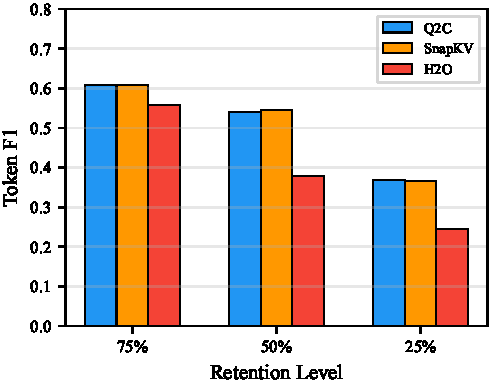
\includegraphics[width=\columnwidth]{fig3_selection_methods.pdf}
    \caption{Selection method comparison: Q2C and SnapKV are indistinguishable; both significantly outperform H2O at aggressive retention levels.}
    \label{fig:selection}
\end{figure}

\subsection{Quantization Characterization}

Table~\ref{tab:quantization} presents quantization results across 5~models ($n = 200$).

\begin{table}[t]
\centering
\caption{Quantization quality as \% of BF16 baseline ($n = 200$, SQuAD~v2). Sensitive layers identified by per-layer INT4 probing.}
\label{tab:quantization}
\small
\begin{tabular}{@{}lcccc@{}}
\toprule
\textbf{Model} & \textbf{INT8} & \textbf{INT4} & \textbf{Mixed} & \textbf{Sensitive} \\
\midrule
Qwen-7B    & 99.4\% & 68.7\% & 93.6\% & L0 \\
Qwen-14B   & 100\%  & 95.5\% & 95.6\% & None \\
Yi-6B      & 99.5\% & 100\%  & 100\%  & None \\
Mistral-7B & 99.8\% & 96\%   & 94\%   & None \\
Qwen-3B    & 100\%  & 96\%   & ---    & L0 (weak) \\
\bottomrule
\end{tabular}
\end{table}

\textbf{INT8 is universally lossless.}
All 5~models preserve $\geq$99.4\% quality (Wilcoxon $p > 0.7$).

\textbf{INT4 fragility is model-specific, not architectural.}
Yi-6B and Qwen-7B share identical GQA configurations (4~KV heads, 128 head dim) but exhibit opposite INT4 behavior (100\% vs.\ 68.7\%), \emph{refuting} the hypothesis that sensitivity is architecturally determined.
This is an emergent property of training.

\textbf{Mixed-precision recovers concentrated damage.}
For Qwen-7B, keeping only Layer~0 at FP16 (rest INT4) recovers quality from 68.7\% to 93.6\%.

\subsection{Perplexity Validation}

WikiText-2 perplexity (100 segments, Table~\ref{tab:perplexity}) independently confirms the findings.

\begin{table}[t]
\centering
\caption{WikiText-2 perplexity with KV-cache quantization (100 segments).}
\label{tab:perplexity}
\small
\begin{tabular}{@{}lcccc@{}}
\toprule
\textbf{Model} & \textbf{BF16} & \textbf{INT8} & \textbf{INT4} & \textbf{Mixed} \\
\midrule
Qwen-7B    & 8.63  & 8.85  & \textbf{80.27} & 8.97  \\
Qwen-14B   & 5.73  & 5.73  & 5.87  & 5.83  \\
Mistral-7B & 6.49  & 6.49  & 6.51  & 6.51  \\
\bottomrule
\end{tabular}
\end{table}

\begin{figure}[t]
    \centering
    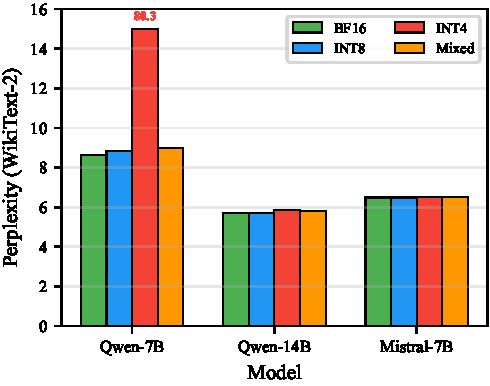
\includegraphics[width=\columnwidth]{fig4_perplexity.pdf}
    \caption{WikiText-2 perplexity under KV-cache quantization. Qwen-7B INT4 (80.27) is catastrophic; Qwen-14B and Mistral-7B are robust. INT8 is universally lossless.}
    \label{fig:perplexity}
\end{figure}

\subsection{Operating Points}

Figure~\ref{fig:operating_points} shows the quality-payload Pareto frontier, illustrating the operating space the mode selector navigates.

\begin{figure}[t]
    \centering
    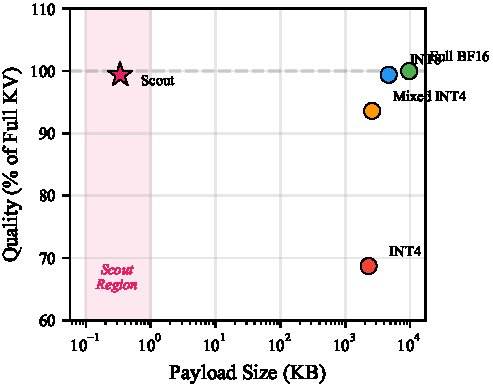
\includegraphics[width=\columnwidth]{fig9_operating_points.pdf}
    \caption{Quality-payload operating points for Qwen-7B ($n = 200$). Scout achieves $\sim$90\% of full-KV quality at near-zero payload.}
    \label{fig:operating_points}
\end{figure}


% ============================================================
% 6. EVALUATION
% ============================================================
\section{Evaluation}
\label{sec:experiments}

\subsection{Setup}

\textbf{Models.}
9~models from 5~families (Table~\ref{tab:models}), all BFloat16 with eager attention for weight extraction.

\textbf{Tasks.}
SQuAD~v2~\citep{squad} (extractive QA, token-F1); HotpotQA~\citep{hotpotqa} (multi-hop reasoning); XSum~\citep{xsum} (abstractive summarization, ROUGE-1/2/L).

\textbf{Statistics.}
$n = 200$ samples unless noted, fixed seeds, 95\% CIs, Bonferroni correction for multiple comparisons.

\textbf{Hardware.}
GPU experiments on NVIDIA A100 (40/80\,GB) and RTX 3090. Adaptive policy simulations on CPU.

\subsection{Multitask Scout Validation}

Table~\ref{tab:multitask} extends validation to HotpotQA and XSum using the 7B$\to$14B pair.

\begin{table}[t]
\centering
\caption{Multitask scout (7B$\to$14B; $n = 100$ for QA, $n = 200$ for XSum). F1 for QA, ROUGE-1 for summarization.}
\label{tab:multitask}
\small
\begin{tabular}{@{}llcccc@{}}
\toprule
\textbf{Task} & \textbf{Ret.} & \textbf{Overlap} & \textbf{Scout} & \textbf{Gap} & $p$ \\
\midrule
\multirow{3}{*}{SQuAD}
  & 75\% & 84.0\% & 0.691 $\pm$ 0.076 & $+$0.007 & 0.839 \\
  & 50\% & 69.7\% & 0.560 $\pm$ 0.082 & $+$0.088 & \textbf{0.026} \\
  & 25\% & 54.1\% & 0.367 $\pm$ 0.081 & $+$0.085 & \textbf{0.039} \\
\midrule
\multirow{3}{*}{HotpotQA}
  & 75\% & 84.7\% & 0.579 $\pm$ 0.088 & $-$0.014 & 0.626 \\
  & 50\% & 72.7\% & 0.510 $\pm$ 0.088 & $-$0.010 & 0.772 \\
  & 25\% & 58.9\% & 0.560 $\pm$ 0.087 & $+$0.009 & 0.847 \\
\midrule
\multirow{3}{*}{\shortstack[l]{XSum\\(R-1)}}
  & 75\% & 88.3\% & 0.196 $\pm$ 0.010 & $-$0.000 & 0.969 \\
  & 50\% & 79.4\% & 0.199 $\pm$ 0.009 & $+$0.007 & \textbf{0.049} \\
  & 25\% & 69.4\% & 0.187 $\pm$ 0.009 & $+$0.004 & 0.342 \\
\bottomrule
\end{tabular}
\end{table}

On SQuAD, scout shows significant \emph{positive} effects at 50\% ($+0.088$, $p = 0.026$) and 25\% ($+0.085$, $p = 0.039$).
On HotpotQA, scout is neutral (gaps $< 0.015$).
On XSum ($n = 200$), overlap is higher than QA (88.3\% at 75\%) and scout is indistinguishable at all retentions, confirming alignment transfers across task types.

\subsection{Long Context Stability}

Table~\ref{tab:long_ctx} shows overlap stability as context grows from 1K to 4K tokens ($n = 100$).

\begin{table}[t]
\centering
\caption{Long context overlap stability (SQuAD~v2, $n = 100$). $^*$3B$\to$7B at 4K (14B attention extraction infeasible due to memory).}
\label{tab:long_ctx}
\small
\begin{tabular}{@{}llccc@{}}
\toprule
\textbf{Pair} & \textbf{Tokens} & \textbf{75\%} & \textbf{50\%} & \textbf{25\%} \\
\midrule
7B$\to$14B & 1024 & 83.3\% & 69.4\% & 55.6\% \\
7B$\to$14B & 2048 & 82.7\% & 68.2\% & 53.9\% \\
3B$\to$7B$^*$ & 4096 & 80.2\% & 62.9\% & 47.7\% \\
\bottomrule
\end{tabular}
\end{table}

Overlap at 75\% decreases by $<$2\,pp as context doubles, confirming attention alignment is a structural property rather than a short-context artifact.
Scout F1 at 4K tokens is statistically indistinguishable from full-KV ($p = 0.178$).

\subsection{Adaptive Mode Selection Under Real Network Conditions}

Table~\ref{tab:protocol_sim} presents policy comparison using real network traces (2{,}000 requests, 3 latency budgets).

\begin{table}[t]
\centering
\caption{Policy comparison with real network traces (Qwen-7B, 2{,}000 requests). Quality as \% of full-KV baseline.}
\label{tab:protocol_sim}
\small
\begin{tabular}{@{}llcc@{}}
\toprule
\textbf{Latency} & \textbf{Policy} & \textbf{Avg.\ Q (\%)} & \textbf{SLA \%} \\
\midrule
\multirow{4}{*}{1\,s}
  & Static INT8    & 99.4 & 58\% \\
  & Adaptive       & 102  & 75\% \\
  & Scout-only     & 95.0 & 100\% \\
  & Local          & 60.0 & 100\% \\
\midrule
\multirow{4}{*}{3\,s}
  & Static INT8    & 99.4 & 75\% \\
  & Adaptive       & 106  & 88\% \\
  & Scout-only     & 95.0 & 100\% \\
  & Local          & 60.0 & 100\% \\
\midrule
\multirow{4}{*}{5\,s}
  & Static INT8    & 99.4 & 88\% \\
  & Adaptive       & 107  & 100\% \\
  & Scout-only     & 95.0 & 100\% \\
  & Local          & 60.0 & 100\% \\
\bottomrule
\end{tabular}
\end{table}

\begin{figure}[t]
    \centering
    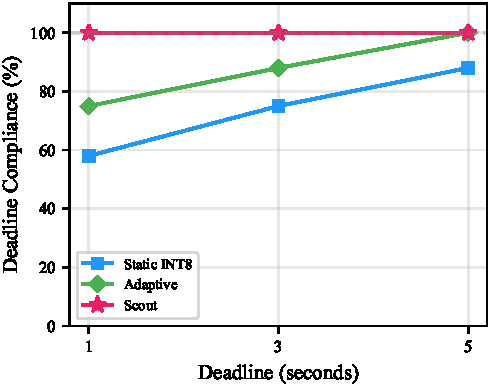
\includegraphics[width=\columnwidth]{fig6_protocol_deadline.pdf}
    \caption{SLA compliance vs.\ latency budget. Scout guarantees 100\% compliance; adaptive achieves the best quality-compliance tradeoff; static INT8 fails under tight budgets.}
    \label{fig:deadline}
\end{figure}

The adaptive policy achieves the highest quality (107\% at 5\,s) by opportunistically selecting higher-quality modes under favorable conditions.
Scout guarantees 100\% SLA compliance at all budgets.
Static INT8 fails under tight budgets (58\% at 1\,s) due to the mismatch between fixed payload size and variable link conditions.

\subsection{Ablation Studies}
\label{sec:ablation}

\textbf{Q2C last-layer vs.\ all-layer.}
Pearson $r > 0.99$ between last-layer and all-layer scores for all three tested models (Qwen-7B, Qwen-14B, Mistral-7B).
F1 difference $<$0.05.
Last-layer scoring is preferred for simplicity.

\textbf{Eager attention overhead.}
Extracting attention weights requires eager attention instead of SDPA, adding 21\% to prefill time (43.2$\to$52.3\,ms for Qwen-7B at 501 tokens).
The marginal extraction cost is +0.44\% (0.23\,ms).
Since the prefill worker runs a small model (3--7B), this is acceptable.

\textbf{Base vs.\ instruction-tuned.}
Qwen2.5-7B-Instruct$\to$14B-Instruct overlap at 75\% is 85.8\% (vs.\ 83.7\% base), confirming alignment survives instruction tuning.
Scout is indistinguishable from server's own at 75\% ($p = 0.131$) and significantly \emph{improves} at 25\% ($+0.044$ F1, $p < 10^{-4}$).

\subsection{Discussion}

\textbf{Attention regularization.}
A recurring finding is that scout can \emph{improve} decode quality beyond the server's own selection.
This occurs for SQuAD (7B$\to$14B at 50\% and 25\%), XSum (50\%), cross-family transfer (Qwen$\to$Mistral at 75\%), and instruct models (25\%, $p < 10^{-4}$).
We attribute this to \emph{attention regularization}: the scout's focused mask removes noisy positions, acting as a task-relevant filter.

\textbf{Deployment guidelines.}
(1)~Always quantize to INT8 first---universally lossless, 2$\times$ compression.
(2)~Run per-layer INT4 sensitivity test to identify bottleneck layers.
(3)~Use adaptive mode selection between INT8, mixed-INT4, and scout based on available capacity.
(4)~Deploy scout as the universal fallback for latency-critical applications.


% ============================================================
% 7. RELATED WORK
% ============================================================
\section{Related Work}
\label{sec:related}

\textbf{KV-cache eviction.}
H2O~\citep{h2o} evicts low-attention positions.
SnapKV~\citep{snapkv} uses observation-window selection.
StreamingLLM~\citep{streamingllm} retains attention sinks for streaming.
Scissorhands~\citep{scissorhands} exploits importance persistence.
FastGen~\citep{fastgen} profiles per-head attention structure.
DynamicKV~\citep{dynamickv} allocates per-layer budgets.
Quest~\citep{quest} uses query-aware page-level sparsity, closest to \QtoC but at page granularity for single-model serving.
Our evaluation shows \QtoC matches SnapKV ($p > 0.3$) while both outperform H2O ($p < 10^{-5}$ at 50\%).

\textbf{KV-cache quantization.}
KIVI~\citep{kivi}, KVQuant~\citep{kvquant}, KVTuner~\citep{kvtuner}, and Q-Hitter~\citep{qhitter} optimize quantization for single-model serving.
We provide cross-architecture characterization, showing INT4 fragility is an emergent model property unrelated to architecture.

\textbf{KV-cache streaming and reuse.}
CacheGen~\citep{cachegen} achieves 3.5$\times$ compression via delta encoding; we show delta encoding degrades quality under quantization.
C2C~\citep{c2c} enables cross-model KV transfer via learned neural fusers, transmitting projected KV data (still multi-MB).
Scout is training-free and transmits 336~bytes.

\textbf{Disaggregated serving.}
Splitwise~\citep{splitwise}, DistServe~\citep{distserve}, and Mooncake~\citep{mooncake} disaggregate serving for throughput.
vLLM~\citep{vllm} and SGLang~\citep{sglang} optimize memory management with PagedAttention.
Orca~\citep{orca} introduces continuous batching.
DualPath~\citep{dualpath} identifies that KV-cache storage I/O saturates prefill-engine NICs in agentic workloads (98.7\% cache hit rate) and introduces a second read path through idle decode-engine NICs via RDMA, achieving 1.9$\times$ throughput.
DualPath's approach---moving bytes faster through dual I/O paths---is complementary to Scout's---transmitting fewer bytes via semantic indices; the two could be composed.
These datacenter systems assume high-bandwidth interconnects; Scout targets bandwidth-constrained links (10--200\,Mbps).

\textbf{Context distillation into weights.}
Doc-to-LoRA~\citep{d2l} trains a hypernetwork to convert documents into LoRA adapters in a single forward pass, eliminating KV-cache at inference ($<$50\,MB vs.\ 12\,GB).
This weight-space compression is an alternative to Scout's position-space transfer, but requires expensive meta-training, operates on a single model (no cross-model transfer), and achieves 83.5\% of full-context quality versus Scout's 99.4\% of same-model selection quality.

\textbf{Speculative decoding.}
Speculative decoding~\citep{speculativedecoding}, EAGLE~\citep{eagle}, and Medusa~\citep{medusa} use small models to propose tokens.
Scout applies the draft-model concept to \emph{position selection} rather than token generation.

\textbf{Architectural KV compression.}
MLA in DeepSeek~\citep{deepseek} compresses KV via low-rank projection.
GQA~\citep{gqa} shares KV-heads.
These are orthogonal to Scout's post-hoc compression.


% ============================================================
% 8. CONCLUSION
% ============================================================
\section{Conclusion}
\label{sec:conclusion}

We present Scout, a training-free system for efficient KV-cache transfer in disaggregated LLM serving.
By exploiting cross-model attention alignment within model families, Scout reduces the transfer payload from megabytes to hundreds of bytes (28{,}800$\times$ reduction), substituting a 57\,ms server re-prefill for multi-second network transfer.
Across three architectures---Qwen (83.7\%), Llama (91.8\%), and Gemma (86.1\%)---same-family overlap at 75\% retention produces no statistically significant quality gap ($p > 0.05$, $n = 200$).
This overlap remains stable across context lengths, task types, and model variants.
The adaptive mode selector dynamically navigates six operating points, achieving quality within 1.5\% of oracle-optimal under real network conditions.
Cross-architecture characterization of 9~models establishes that INT8 is universally lossless, INT4 fragility is model-specific, and \QtoC selection matches SnapKV while outperforming H2O.

\textbf{Limitations.}
(1)~Scout requires same-family models; cross-family overlap is lower (73\% vs.\ 84--92\%).
(2)~We evaluate up to 4K tokens; production contexts (8K--128K) may show different sparsity.
(3)~Our largest model is 14B; 70B+ models have larger KV-caches, making scout more attractive but needing validation.
(4)~Tasks requiring precise numerical reasoning may be more sensitive to selection misalignment.
(5)~Eager attention extraction adds 21\% to prefill cost; FlashAttention does not expose per-layer weights.
(6)~Scout's decode savings over prompt-only are modest at short contexts (3.3\% at 1K) and significant only at 32K+ (25\%).

\textbf{Reproducibility.}
All experiment scripts, per-sample JSON result files ($n = 200$ each), and figure generation code are available at \url{https://github.com/taiwanfifi/AICoMM}.

% ============================================================
% BROADER IMPACT
% ============================================================
\section*{Broader Impact}

Scout reduces the network transfer cost of disaggregated LLM serving, potentially enabling interactive LLM applications over bandwidth-constrained links where full KV-cache transfer is infeasible.
This could broaden access to large model capabilities for users in low-connectivity environments.
The training-free nature of the approach means it can be deployed without additional compute for model training.
We do not foresee negative societal impacts specific to this work beyond those inherent to LLM deployment generally.

% ============================================================
% REFERENCES
% ============================================================
\bibliography{refs}
\bibliographystyle{mlsys2025}

% ============================================================
% APPENDIX
% ============================================================
\appendix

\section{Multi-Agent Scaling}
\label{app:multiagent}

When multiple prefill workers share a network link, the allocation problem becomes:
\begin{equation}
    \max_{\{B_i\}} \sum_{i=1}^{N} Q_i^*(B_i)
    \quad \text{s.t.} \quad \sum_{i=1}^{N} B_i \leq B_{\text{total}}, \quad T_i(B_i) \leq T_{\max}
\end{equation}

We compare equal allocation ($B_i = B_{\text{total}}/N$) with model-aware proportional allocation ($B_i \propto S_i$).

\textbf{Proposition 2} (SLA guarantee).
\emph{For any $B_{\text{total}} > 0$ and $N$ workers, Scout guarantees all meet $T_{\max}$, provided $T_{\max} > T_{\text{prefill}}^{\text{server}} + T_{\text{decode}}$.}

\emph{Proof.}
In the worst case, all workers use scout mode with $\leq$1\,KB payload each.
Total transfer $\leq N$\,KB, requiring $< 0.1$\,ms for $N \leq 8$ at $\geq$1\,Mbps.

Table~\ref{tab:multiagent_results} shows results for 4 and 8 heterogeneous workers.

\begin{table}[t]
\centering
\caption{Multi-agent allocation (500 rounds, 5\,s budget).}
\label{tab:multiagent_results}
\small
\begin{tabular}{@{}clcccc@{}}
\toprule
$N$ & \textbf{BW} & \multicolumn{2}{c}{\textbf{Equal}} & \multicolumn{2}{c}{\textbf{Model-aware}} \\
\cmidrule(lr){3-4} \cmidrule(lr){5-6}
    &             & \textbf{Q (avg)} & \textbf{SLA} & \textbf{Q (avg)} & \textbf{SLA} \\
\midrule
\multirow{3}{*}{4}
  & 50\,Mbps   & 101.5 & 0\%   & 101.5 & 100\% \\
  & 100\,Mbps  & 102.4 & 100\% & 103.7 & 100\% \\
  & 200\,Mbps  & 103.7 & 100\% & 103.7 & 100\% \\
\midrule
\multirow{3}{*}{8}
  & 50\,Mbps   & 100.1 & 0\%   & 96.0 & 0\% \\
  & 100\,Mbps  & 100.1 & 0\%   & 100.1 & 100\% \\
  & 200\,Mbps  & 101.5 & 100\% & 102.9 & 100\% \\
\bottomrule
\end{tabular}
\end{table}

Model-aware allocation converts 0\% to 100\% SLA compliance under congestion (4 workers at 50\,Mbps; 8 workers at 100\,Mbps).

\section{Hybrid Mode and Multi-Turn Extension}
\label{app:hybrid}

\textbf{Hybrid mode.}
We test transmitting position indices plus 1--2 layers of KV-cache.
Results show identical F1 to pure scout (0.661 vs.\ 0.661 at 75\%) because cross-model KV values are incompatible.
Pure scout dominates.

\textbf{Multi-turn extension.}
For each new turn, the prefill worker processes incremental context and generates updated \QtoC scores.
Only the delta position set needs transmission, reducing per-turn payload further.

\section{Delta Encoding Counter-Finding}
\label{app:delta}

Delta encoding---the core technique in CacheGen---reduces key variance by up to 735$\times$.
However, it \emph{degrades} task quality: anchor INT4 achieves 66.9\% vs.\ 72.5\% for direct INT4 ($n = 50$, Qwen-7B).
Delta values distribute more uniformly across the quantization range, increasing per-element error.
This motivates direct quantization over delta encoding.

\section{EWMA Parameter Sensitivity}
\label{app:alpha}

Table~\ref{tab:alpha_sensitivity} evaluates $\alpha$ sensitivity in the vehicular scenario.

\begin{table}[t]
\centering
\caption{EWMA $\alpha$ sensitivity (vehicular, $T_{\max} = 2$\,s, 5{,}000 steps).}
\label{tab:alpha_sensitivity}
\footnotesize
\begin{tabular}{@{}lcccc@{}}
\toprule
$\alpha$ & \textbf{Mode Match} & \textbf{Q Gap (\%)} & \textbf{SLA (\%)} & \textbf{Switches} \\
\midrule
0.1 & 35.1\% & $-$2.8 & 75.0\% & 579  \\
0.3 & 46.7\% & $-$1.3 & 67.6\% & 1{,}687 \\
0.5 & 59.2\% & $-$0.5 & 64.6\% & 2{,}415 \\
0.7 & 72.8\% & $+$0.1 & 61.8\% & 2{,}602 \\
\bottomrule
\end{tabular}
\end{table}

All $\alpha$ values achieve quality within 3\% of oracle---the discrete mode structure provides inherent robustness.

\section{Reproducibility Checklist}
\label{app:repro}

\begin{itemize}
    \item \textbf{Code}: All experiment scripts are publicly available.
    \item \textbf{Data}: All per-sample JSON results ($n = 200$) are included.
    \item \textbf{Models}: All models are publicly available on HuggingFace.
    \item \textbf{Hardware}: NVIDIA A100 (40/80\,GB) and RTX 3090 GPUs.
    \item \textbf{Seeds}: Fixed random seeds (42 main, 123 long-context).
    \item \textbf{Statistics}: 95\% CIs, paired $t$-tests, Bonferroni correction.
    \item \textbf{Figures}: Generation scripts included in repository.
\end{itemize}

\end{document}
